\documentclass[11pt]{beamer}
\usetheme{Dresden}
%\usecolortheme{beaver}
\usepackage[utf8]{inputenc}
\usepackage{amsmath}
\usepackage{amsfonts}
\usepackage{amssymb}
\usepackage{graphicx}
\usepackage{listings}
\usepackage{verbatim}
\author{Zheng Zheng}
\title{Topic 1 - Shell Basics}
%\setbeamercovered{transparent} 
%\setbeamertemplate{navigation symbols}{} 
%\logo{} 
\institute{McMaster University}
\date{Winter 2023} 
\subject{COMPSCI 1XC3 - Computer Science Practice and Experience:
Development Basics} 
\stepcounter{section}

\definecolor{mGreen}{rgb}{0,0.6,0}
\definecolor{mGray}{rgb}{0.5,0.5,0.5}
\definecolor{mPurple}{rgb}{0.58,0,0.05}
\definecolor{mGreen2}{rgb}{0.05,0.65,0.05}
\definecolor{mGray2}{rgb}{0.55,0.55,0.55}
\definecolor{mPurple2}{rgb}{0.63,0.05,0.05}
\definecolor{backgroundColour}{rgb}{0.95,0.95,0.92}
\definecolor{backgroundColour2}{rgb}{0.95,0.92,0.95}

\let\OldTexttt\texttt
\renewcommand{\texttt}[1]{\OldTexttt{\color{teal}{#1}}}

\lstdefinestyle{C}{
    backgroundcolor=\color{backgroundColour},   
    commentstyle=\color{mGreen},
    keywordstyle=\color{blue},
    numberstyle=\tiny\color{mGray},
    stringstyle=\color{mPurple},    
    basicstyle=\footnotesize,
    breakatwhitespace=false,         
    breaklines=true,                 
    captionpos=b,                    
    keepspaces=true,                 
    numbers=left,                    
    numbersep=5pt,                  
    showspaces=false,                
    showstringspaces=false,
    showtabs=false,                  
    tabsize=2,
    language=C
}

\definecolor{eggplant}{rgb}{0.52,0.11,0.3} 

\usecolortheme[named=eggplant]{structure}

\begin{document}

\begin{frame}
\center
COMPSCI 1XC3 - Computer Science Practice and Experience:
Development Basics
\titlepage
% Toggle for C chapters
% Adapted from C: How to Program 8th ed., Deitel \& Deitel
\end{frame}

\begin{frame}
\tableofcontents
\end{frame}

\section[History]{A Brief History of Computing}
\begin{frame}{The First Generation Computers}
Computers (based on vacuum tubes) were very large, requiring large rooms for their housing. Programming via machine instructions, assembly language.
\center
\includegraphics[scale=0.1]{eniac.jpg} \\
ENIAC (Electronic Numerical Integrator and Computer) was the first programmable, electronic, general-purpose digital computer, completed in \emph{1945}.
\end{frame}

\begin{frame}{Semiconductor Electronics and Integrated Circuits (IC)}
\begin{itemize}
    \item The semiconductor transistor (late 40s) is possibly the most important invention of the $20^{th}$ century. It has smaller size, longer life and higher efficiency (100X).
    \item From late 1950s to 1960s, the development of IC contributed to the birth of the $3^{rd}$ generation computers.
    \item Moore's law is the observation that the number of transistors in a dense IC doubles about every two years.
\end{itemize}
% The exponential growth of the number of transistors per unit area over time meant that by the mid seventies, the home or personal microcomputer began outpacing the mainframe in terms of computational power.  
\center
\includegraphics[scale=0.3]{microchip.jpg}
\end{frame}

\begin{frame}{Distinctive feature of third-generation computers}
\begin{itemize}
    \item Gradual maturity of the operating system (OS).
    \item Advanced Programming Languages.
    \begin{itemize}
        \item Programs written at this time (notably using FORTRAN, COBOL and LISP) were not generally portable between machine architectures. \texttt{Incompatible due to a lack of standardization!}
        
        \item All this changed with the development of C in 1972 by Dennis Ritchie at Bell laboratories.
        \begin{itemize}
            \item Because C was strongly standardized, C programs could be ported across participating computer architectures with no compatibility issues.
            \item C was originally developed for writing utilities for the Unix operating system.
        \end{itemize}
    \end{itemize}
\end{itemize}

\end{frame}

\begin{frame}{Unix - the Uniplexed Information and Computing Service}
\begin{itemize}
\item Unix was originally written in assembly code, but after the development of C, the Bell Labs gang re-implemented the Unix kernel in C, and it has remained in C ever since.  
\item Due to it's low cost and high portability (especially to low-cost hardware), Unix was widely adopted by academic institutions, and from there, \emph{the world!}
\item Unix featured some key innovations: 
    \begin{itemize}
        \item An hierarchical file system with arbitrarily nested sub-directories
        \item The universalization of almost all file formats as new-line delimited plain text.  
        \item A pervasive philosophy of modularity and code re-use, and the establishment of a set of cultural norms for software development practice.   
    \end{itemize}
\end{itemize}
\end{frame}

\begin{frame}{The Unix Family}
\center
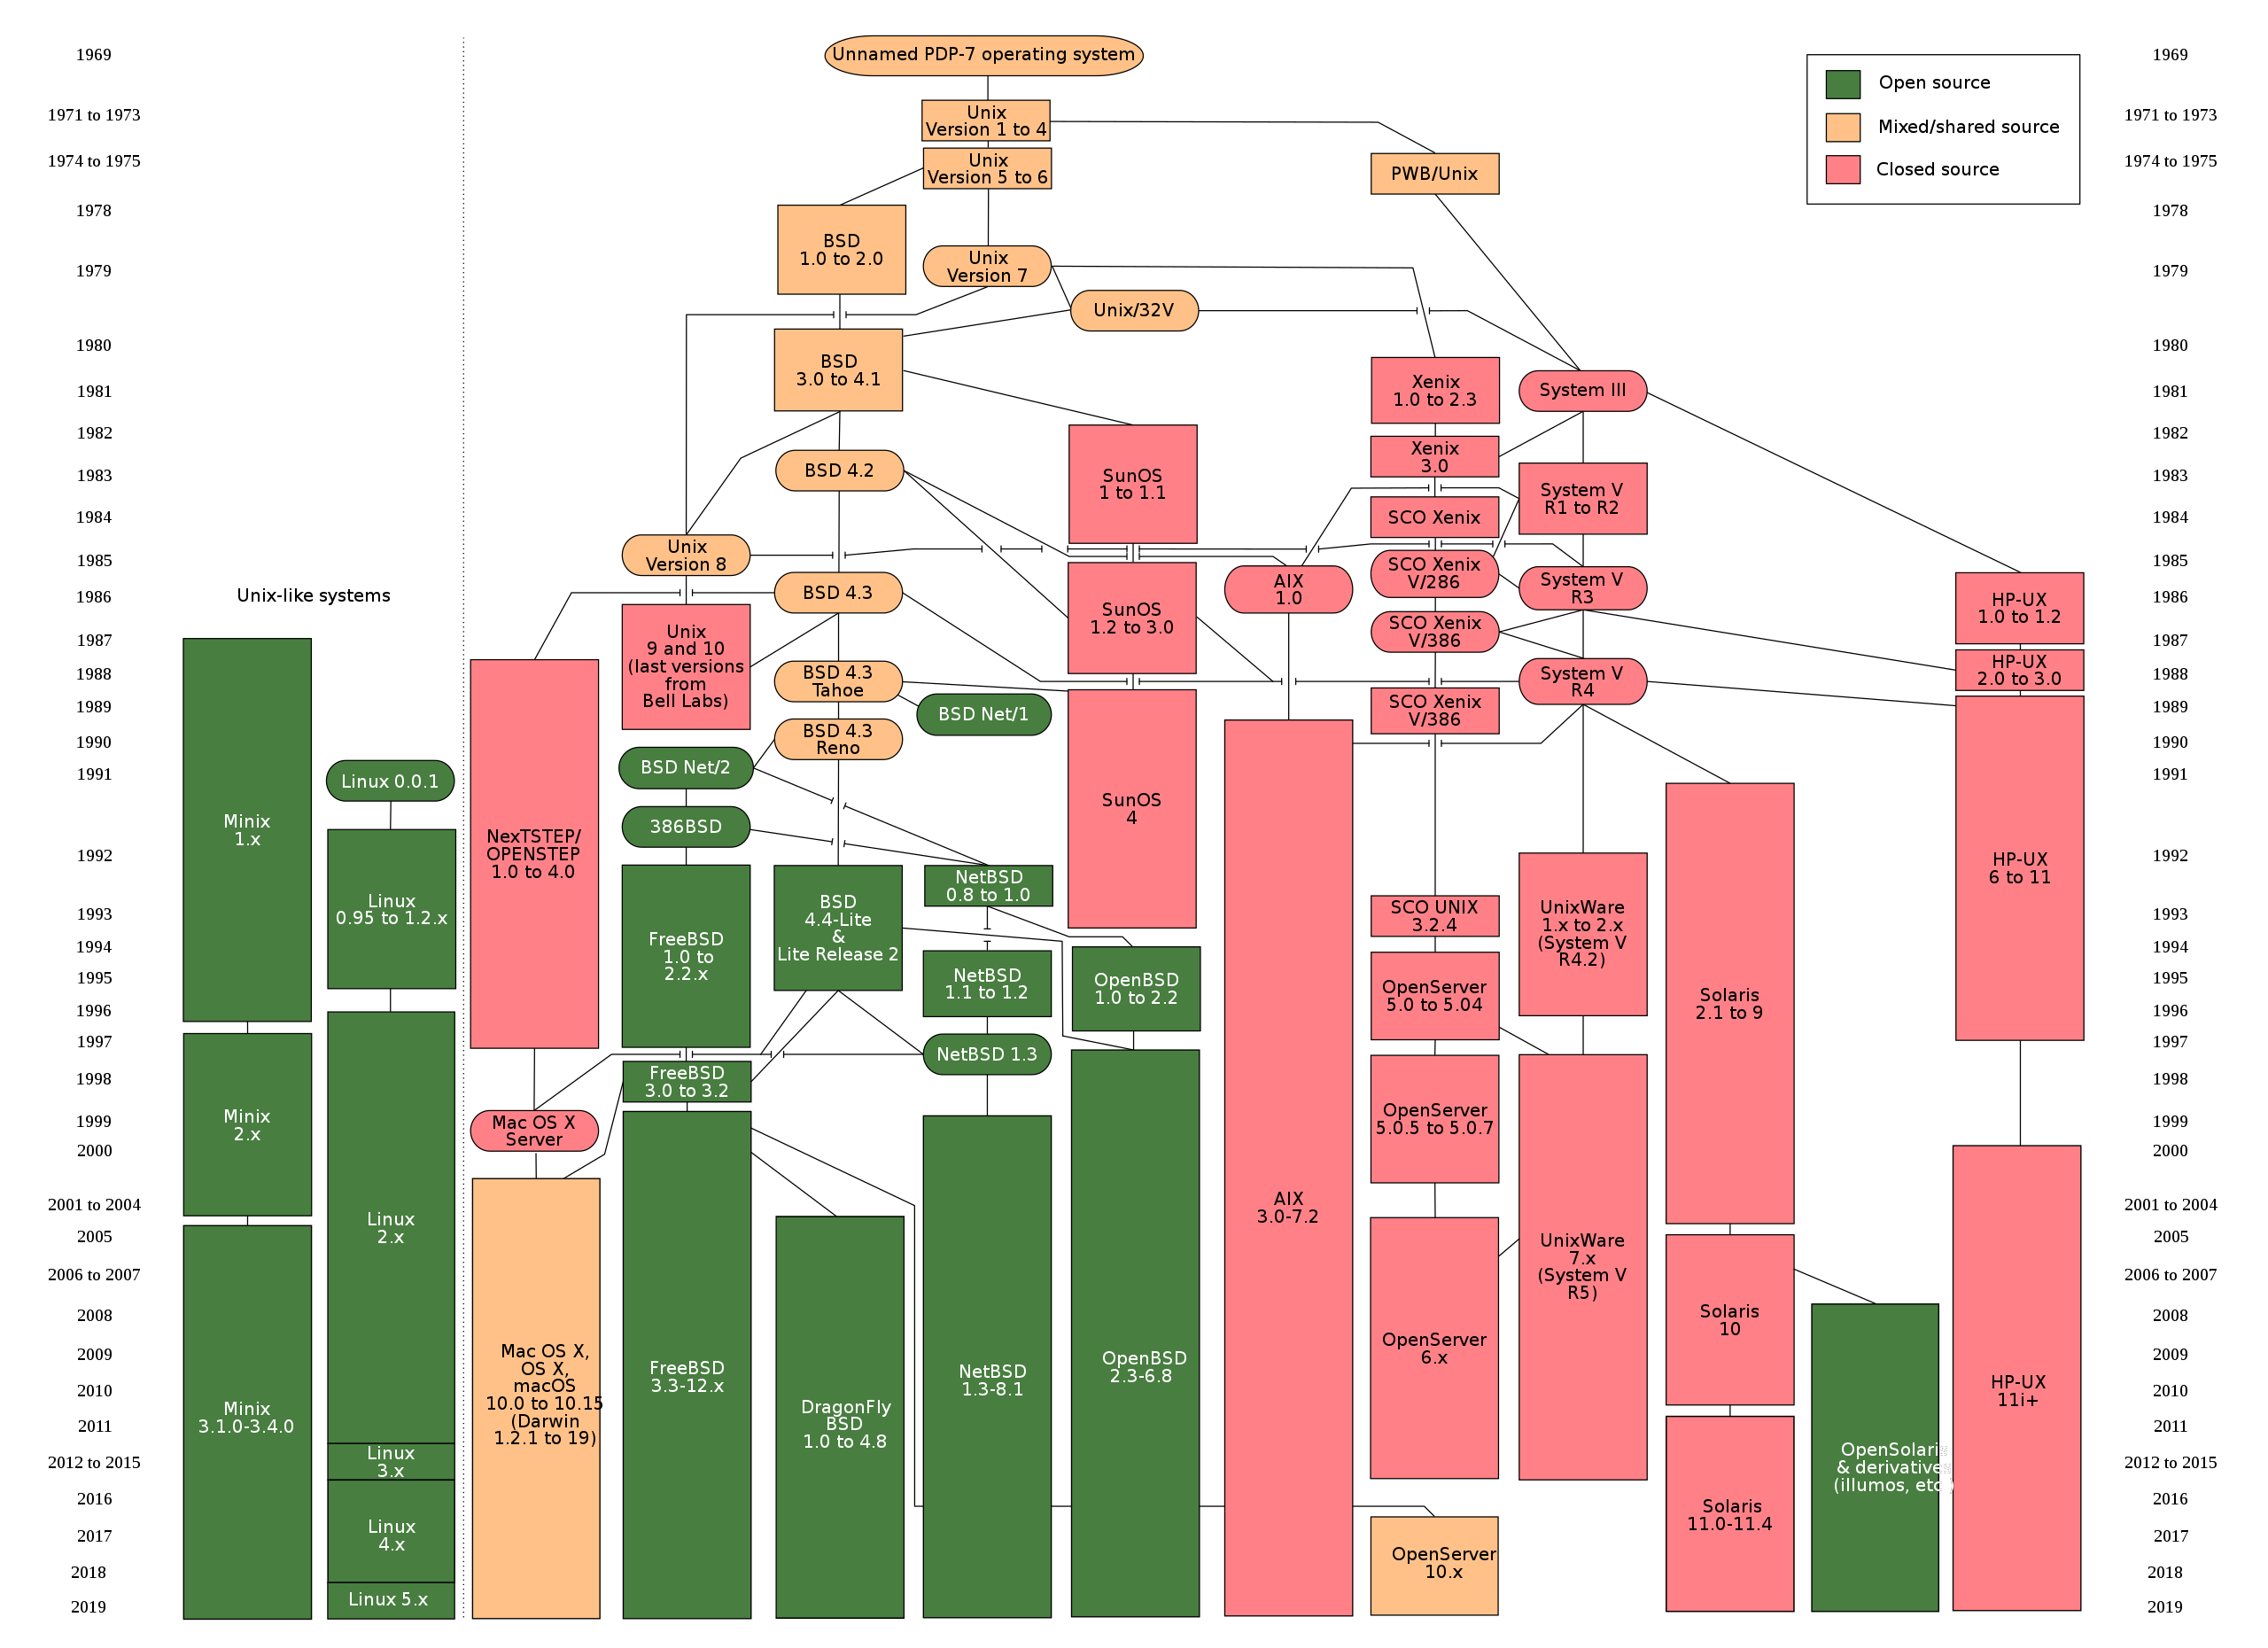
\includegraphics[scale=0.1]{unixfamily.png}
\end{frame}

\section[Operating Systems]{Operating Systems}
\begin{frame}{Operating Systems}
\center
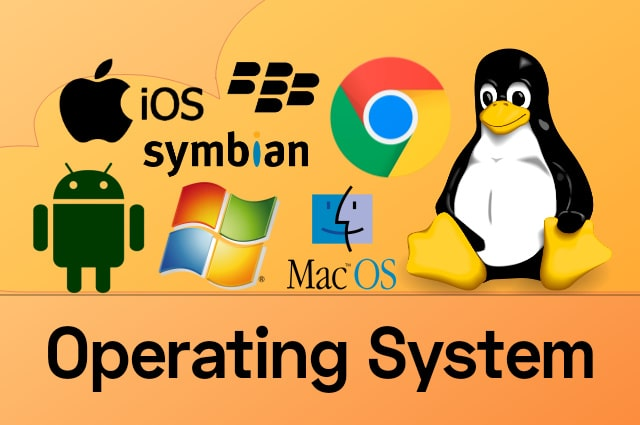
\includegraphics[scale=0.35]{OS.jpeg}
\end{frame}

\begin{frame}{Operating Systems In General}
\begin{columns}
\begin{column}{.5\textwidth}
An \textbf{Operating System} provides a collection of services to \textbf{User Applications}, allowing them to run on a computer system's \textbf{hardware}.  
\begin{itemize}
\item User Applications are anything from internet browsers to word processors to solitaire.
\item The \textbf{API} provides system libraries and other utilities via \emph{system calls}.
\begin{itemize}
\item These are typically executed by the \textbf{Kernel}. 
\end{itemize}
\end{itemize}
\end{column}
\begin{column}{.5\textwidth}
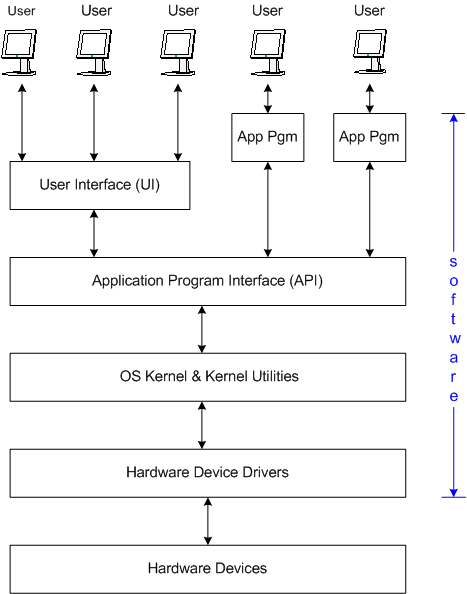
\includegraphics[scale=0.3]{op_sys_block_diagram.png}
\end{column}
\end{columns}
\end{frame}

\begin{frame}{The Kernel}
\begin{columns}
\begin{column}{0.5\textwidth}
Operating systems include a \textbf{kernel}, which manages:
\begin{itemize}
\item Access to Memory (Random Access and Read Only)
\item Access to the CPU
\item Input / Output handling
\item Access to hardware and software resources
\end{itemize}
Most operating systems use kernels written in C, because C is \emph{fast}.
\end{column}
\begin{column}{0.5\textwidth}
\includegraphics[scale=0.2]{shells.png}
\end{column}
\end{columns}
\end{frame}

\begin{frame}{Linux}
Linux is a family of free operating systems.
\begin{columns}
\begin{column}{0.25\textwidth}
\includegraphics[scale=0.4]{Tux.png}
\end{column}
\begin{column}{0.73\textwidth}
\begin{itemize}
\item Unix was free until 1984 when AT\&T divested itself of Bell Labs.  Unix then became proprietary software. 
\item This led to the creation of The GNU Project, and the GNU General Public License in 1989, which kicked off the \emph{open source} movement.  
\item The Linux Kernel was written in 1991 by Linus Torvalds at the University of Helsinki.
\end{itemize}
\end{column}
\end{columns}
\vspace{0.5em}
Today, Linux has the largest install base of any operating system, though only about 2\% of personal computers run it. 
\end{frame}

\section[Using a Command Line]{Bash}
\begin{frame}{Giving it a Bash!}
In Linux distributions, command line interfaces are commonly used
\begin{itemize}
\item Command lines have a high skill cap than Graphical User Interface (GUI).  
\end{itemize}
The \textbf{Bash} shell is a very common command line interface in Unix-like environments.
\begin{itemize}
\item In Windows:
	\begin{itemize}
	\item The Windows Subsystem for Linux allows Windows 10 users to access a bash prompt. 
	\end{itemize}
\item On Macintoshes:
	\begin{itemize}
	\item Opening up a terminal and entering the command \texttt{bash}
	\end{itemize}
\item In Linux:
	\begin{itemize}
	\item Do you have to ask? 
	\end{itemize}
\end{itemize}
This course will require you to have ready access to a bash prompt.  \textbf{Your homework this week is to get your computer set up so that you have access to a bash prompt.}  
\end{frame}

\begin{frame}{Accessing Linux from Older Windows Computers}
We have set up a server for you to login to if the options on the previous slide don't work.  
\begin{itemize}
\item Remote servers are accessed using a \textbf{Secure Shell Protocol (SSH)}.  
\item On Windows, it is common to use a secure shell client, such as \textbf{PuTTY}.
\begin{itemize}
\item \url{https://www.chiark.greenend.org.uk/~sgtatham/putty/}
\end{itemize}
\end{itemize}
The department has set up a server for the class to use this semester.  For more information on how to access it, check the \emph{Resources} section of the course content on Avenue.
\begin{itemize}
\item Always remember to \texttt{logout} when you're finished! 
\end{itemize}
\end{frame}

\begin{frame}{Bash Commands}
Almost all Unix and Unix-like systems support a comprehensive set of Bash commands.
\begin{itemize}
\item \url{https://en.wikipedia.org/wiki/List_of_Unix_commands}
\end{itemize}
Bash commands are extremely versatile.
\begin{itemize}
\item The output of one command can be made the input of another command using \textbf{Pipes and Filters}
\item Bash commands can be collected into \textbf{Scripts} and executed as units.
\item Bash commands can be invoked from programs written in C or Python.
\end{itemize}
All these topics will be covered in this course.
\end{frame}

\begin{frame}[fragile=singleslide]{Directory Structure}
The directory structure in Linux is \textbf{hierarchical}.
\begin{itemize}
\item Directories may contain files and sub-directories, forming a \textbf{tree}.  
\end{itemize}
In Bash, commands are executed within the \textbf{working} or \textbf{active directory}.  
\begin{itemize}
\item One directory in your file system is designated as \emph{active}.  This active directory may be changed using the \texttt{cd} command.  
\end{itemize}
\begin{lstlisting}[style=C, language=bash]
%user@system:~/Documents/Example $ cd Topic1
%user@system:~/Documents/Example/Topic1 $ cd ..
%user@system:~/Documents/Example/ $ cd ..
%user@system:~/Documents/ $ cd Example/Topic2
%user@system:~/Documents/Example/Topic2 $ cd 
\end{lstlisting}

\end{frame}


\begin{frame}{Actual Bash Commands}
\begin{tabular}{|| l || c |}
\hline 
Command & Description \\ \hline
\texttt{cat <filename>} & display the contents of the file \\ \hline
\texttt{cd <directory>} & change the working directory \\ \hline
\texttt{cp <filename> <filename>} & copy a file \\ \hline
\texttt{ls} & List directory contents \\ \hline
\texttt{man <command>} & show a command's \textbf{man page} \\ \hline
\texttt{mkdir <directory>} & make directory \\ \hline
\texttt{ps} & list all processes \\ \hline
\texttt{pwd} & outputs current working directory \\ \hline
\texttt{rm <filename>} & removes a file \\ \hline
\texttt{rmdir <directory>} & removes a directory (if empty) \\ \hline
% \texttt{grep ...} & search file contents \\ \hline
\end{tabular}
Important Linux Commands: https://www.howtogeek.com/412055/37-important-linux-commands-you-should-know/
\end{frame}


\section[Network Protocols]{Network Protocols}
\begin{frame}[fragile=singleslide]{Secure Shell Protocol}
\begin{lstlisting}[language = bash, style = C]
 $ ssh username@serverURLaddress.com 
\end{lstlisting}
The Secure Shell (SSH) protocol is a network protocol for secure remote login over insecure networks.
\begin{itemize}
\item A \textbf{network protocol} is an agreed-upon format for information transmission.
\item Anything but military-grade intranet should be considered insecure... 
	\begin{itemize}
	\item And even then...
	\end{itemize}
\end{itemize}
In short, you (the \textbf{client}) open a shell on a remote \textbf{server}.  
\begin{itemize}
\item This is the way that PuTTY accesses $pascal.cas.mcmaster.ca$, it just gives you a nice little GUI for entering the connection details.
\end{itemize}
\end{frame}

\begin{frame}{Graphical User Interface (GUI)}
\begin{columns}
\begin{column}{0.6\textwidth}
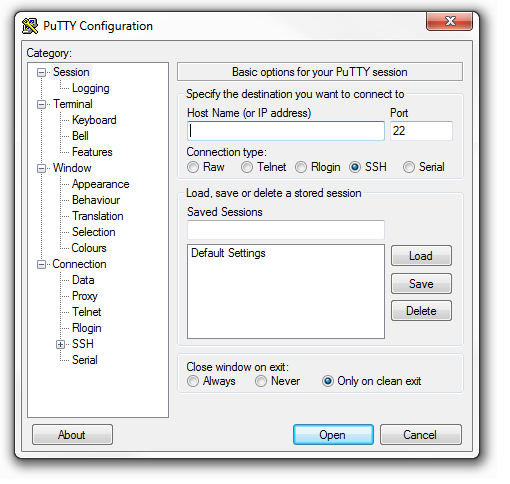
\includegraphics[scale=0.4]{putty.png}
\end{column}
\begin{column}{0.38\textwidth}
The point of this course is for you to gain computer skills. \\ 
\vspace{0.5em}
The most important computer skill is knowing when and how to look things up. \\
\vspace{0.5em}
When in doubt, consult the documentation! 
\end{column}
\end{columns}
\end{frame}

% \begin{frame}
% \center
% 
\includegraphics[scale=0.46]{obiwan.jpg}
% \end{frame}

\begin{frame}{Network Protocols}
Some common network protocols:
\begin{itemize}
\item Ethernet
\item Internet Protocol (IP)
\item Transmission Control Protocol (TCP)
\item Hypertext Transfer Protocol (HTTP)
\item Dynamic Host Configuration Protocol (DHCP)
\end{itemize}
Network protocols typically define the construction of  \textbf{data packets}, which are transferred by the network.
\begin{itemize}
\item In general, data packets consist of a \textbf{header}, followed by some data.  
\item The header may contain different information depending on the protocol, such as the size of the packet, the source and destination of that packet, and security features like check-sums.  
\end{itemize}
\end{frame}

\begin{frame}{Header Organization for IPv6 Data Packet}
\center
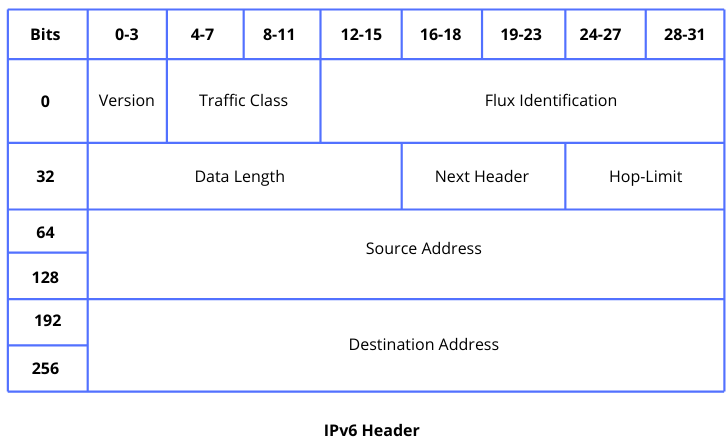
\includegraphics[scale=0.32]{IPV6-header.png} \\
In general, the exact construction of data packets isn't something you need to worry about unless you're a network specialist or an Electrical Engineer.  
\end{frame}

% \section[Errata]{Errata}
% \begin{frame}{The Last Slide Comic}
% 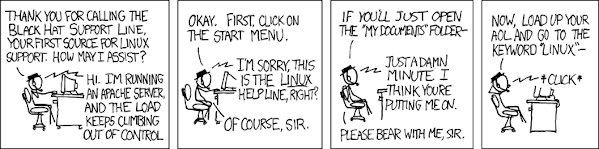
\includegraphics[scale=0.5]{black_hat_support.png}
% \end{frame}

\section[Acknowledge]{Acknowledge}
\begin{frame}{Acknowledge}
\center
\vspace{8em}
The contents of these slides were liberally borrowed (with permission) from slides from the Summer 2021 offering of 1XC3 (by Dr. Nicholas Moore).  
\end{frame}

\end{document}
